\section{Uses of Zcash}

Zcash can be used as a speculative investment tool and/or as a form of payment. When used as a speculative investment tool, the actual profit from the investment can vary over time depending on the fluctuation of Zcash's price, as the cryptocurrency market is highly volatile. Nevertheless, the most interesting use is as a form of payment, as Zcash allows for transactions where amounts, recipients, and senders remain \textbf{anonymous}. This feature makes Zcash popular for payments on the \textbf{Dark Web}.

\subsection{Zcash on the Dark Web}

The Deep Web is everything that is not visible on search engines, while the Dark Web refers to Deep Web content accessible via the internet through specific software, configurations, and authorization. On the Dark Web, a vast amount of products and services, both legal and illegal, can be purchased.

\noindent Payments on the Dark Web are made with cryptocurrencies due to their decentralization and, most importantly, the privacy guarantees they offer. The most used cryptocurrencies on the Dark Web are Monero, Dash, Litecoin, Bitcoin (even though Bitcoin's privacy is not correctly guaranteed), but also Zcash itself.

\noindent According to research conducted by the RAND Corporation \cite{rand}, there is some \textbf{possible evidence} indicating that Zcash may be used for:
\begin{itemize}
    \item \textbf{Money laundering}: Zcash is particularly suitable for money laundering, as every single financial transaction is impossible to trace and identify;
    \item \textbf{Payments for purchasing illegal goods and services}: various studies show that Zcash is accepted as a form of payment on the Dark Web;
    \item \textbf{Terrorist financing}: it has been discovered that a Telegram account titled “Supporto tecnico della Fondazione Afaq Electronic Foundation,” a media group associated with ISIS, advised followers to use Zcash instead of Bitcoin for transactions directed to the group.
\end{itemize}

\noindent On the Dark Web, various e-commerce platforms sell diverse services and products. The most well-known is certainly \textbf{Dream}, but it is not the only one (Figure \ref{fig:e-commerce}). Many e-commerce platforms, such as the \textbf{Berlusconi} e-commerce, were later shut down, but they still marked an important gathering point for criminals for years.

\noindent The most sold services, goods, and products on various Dark Web e-commerce platforms are drugs, frauds, digital goods, but also weapons and jewelry.

\begin{figure}[!ht]
    \centering
    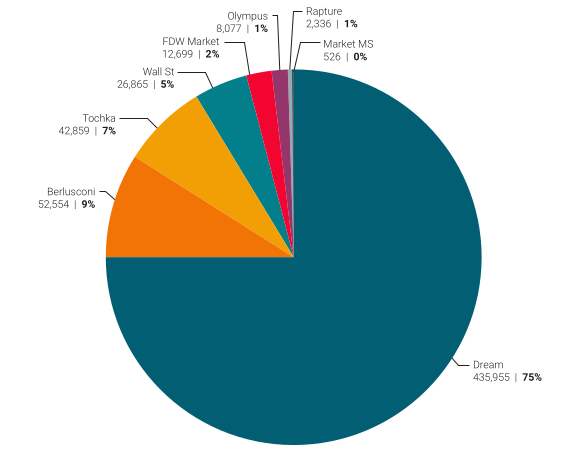
\includegraphics[width=1\linewidth]{img/eCommerce.png}
    \caption{E-commerce on the Dark Web}
    \label{fig:e-commerce}
\end{figure}

\noindent Multiple cryptocurrencies are used for purchases. The most used is Bitcoin, followed by Monero and Ethereum. Zcash is, along with Litecoin, one of the less used currencies for payments. A summary of the payment distribution is presented in Figure \ref{fig:cryptoPayments}.

\begin{figure}[!ht]
    \centering
    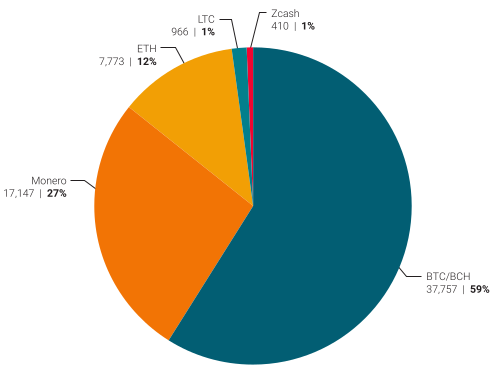
\includegraphics[width=1\linewidth]{img/cryptoPayments.png}
    \caption{Cryptocurrencies used for making payments}
    \label{fig:cryptoPayments}
\end{figure}

\noindent Further research indicates that Zcash is mentioned as an accepted payment form primarily by three sellers:
\begin{itemize}
    \item \textbf{TheShop};
    \item \textbf{Skyscraper};
    \item \textbf{Cyberzen}.
\end{itemize}

\noindent Although Zcash is potentially suitable for handling transactions related to the purchase of illegal goods and/or services, its use is still limited. The reason is simple: Zcash was created as a cryptocurrency that aims to ensure privacy, not to facilitate untraceable illegal payments, but to offer an additional form of protection to the end user in terms of traceability. Monero, for example, is a cryptocurrency created with the intent of becoming the most widespread form of payment on the Dark Web from the very beginning.

\noindent In conclusion, Zcash represents a significant evolution in the cryptocurrency landscape, combining blockchain security with transaction privacy.